\chapter{Time Aggregation in Panel Data on Income and Consumption}

\section{Abstract}
In 1960 Working noted that time aggregation of a random walk induces serial correlation in the first differences that is not present in the original series. This important contribution has been overlooked in a large recent literature analyzing income and consumption in panel data. This paper takes \cite{blundell_consumption_2008} as an example and shows how to correct for this problem. I find the estimate for the partial insurance to transitory shocks, originally estimated to be 5\%, is equal to 24\% when corrected for time aggregation. This estimate is much closer to estimates from the literature that uses natural experiments to estimate the marginal propensity to consume out of transitory shocks.

\section{Introduction}
In a short note in Econometrica, \cite{working_note_1960} made the simple but important point that time aggregation can induce serial correlation that is not present in the original series. This fact was readily absorbed by the macroeconomic literature, where such time aggregated series are common (for an example see \cite{campbell_consumption_1989}). Recently, by studying the covariance structure of panel data, much progress has been made in understanding household income and consumption dynamics. However, this literature has not accounted for the serial correlation induced by the time aggregated nature of observed income and consumption data. This oversight can result in significant bias. This paper will focus on the implications of time aggregation for the methodology in \cite{blundell_consumption_2008} (henceforth BPP), but it applies to a broad swath of the literature. I show that the pass through from transitory income to consumption, originally estimated by BPP to be 5\%, is close to 25\% when the serial correlation in the data induced by time aggregation is accounted for.

\subsection{What is Time Aggregation?}
Many observed time series in economics are given at a lower frequency than the underlying data that generates them. For example, income is often observed at an annual frequency when it may in fact consist of paychecks arriving at a monthly, biweekly or irregular timetable. To transform income into an annual frequency we sum up all the income that was received by a household during the year, a process known as time aggregation. The key insight of \cite{working_note_1960} is that even if there is no correlation between changes in income at the underlying frequency, the resulting time aggregated series will show positive autocorrelation. The intuition behind this can be seen in figure \ref{fig:TimeAggExample} showing an income process that begins at zero and increases to one in the second year. The top left graph shows the path of income if the shock occurs exactly at the start of the second year, and the bottom left graph shows the time aggregated process exactly mirrors that. There is no income in the first year and one unit of income in each of the second and third years. The top right shows an alternative income process in which the shock occurs half way through the second year. Now the resulting time aggregated process (bottom right) does not mirror the underlying. As before there is no income in the first year, but in the second year the individual receives an income of one for half the year, resulting in a time aggregated income of 0.5. In the third year the individual receives an income of one for the entire year, and hence a time aggregated income of one. If we can only see the time aggregated process, when we observe income increasing from year one to year two we do not know if the shock occurred at the beginning of the year or half way through. If it occurred at the beginning of the year, as in the left hand graphs of figure \ref{fig:TimeAggExample}, then we would not expect to see any further increase in the time aggregated process associated with it. However, if it occurred half way through, as in the right hand graphs of figure \ref{fig:TimeAggExample}, we would only have observed half the total increase in income and would expect the time aggregated process to continue to increasing in the following period. Therefore, assuming there is some positive probability that the shock occurred half way through the second period, we would expect to see further increases in the observed process. This is how time aggregation induces serial correlation in the first difference of an observed process even when the underlying process is a random walk. Section \ref{TimeAggRandomWalk} lays this out formally and shows that this autocorrelation tends to $\frac{1}{4}$ as the number of time subdivisions increases to infinity.
\begin{figure}
%	\caption{Time Aggregation Induces Serial Correlation}
	\label{fig:TimeAggExample}
	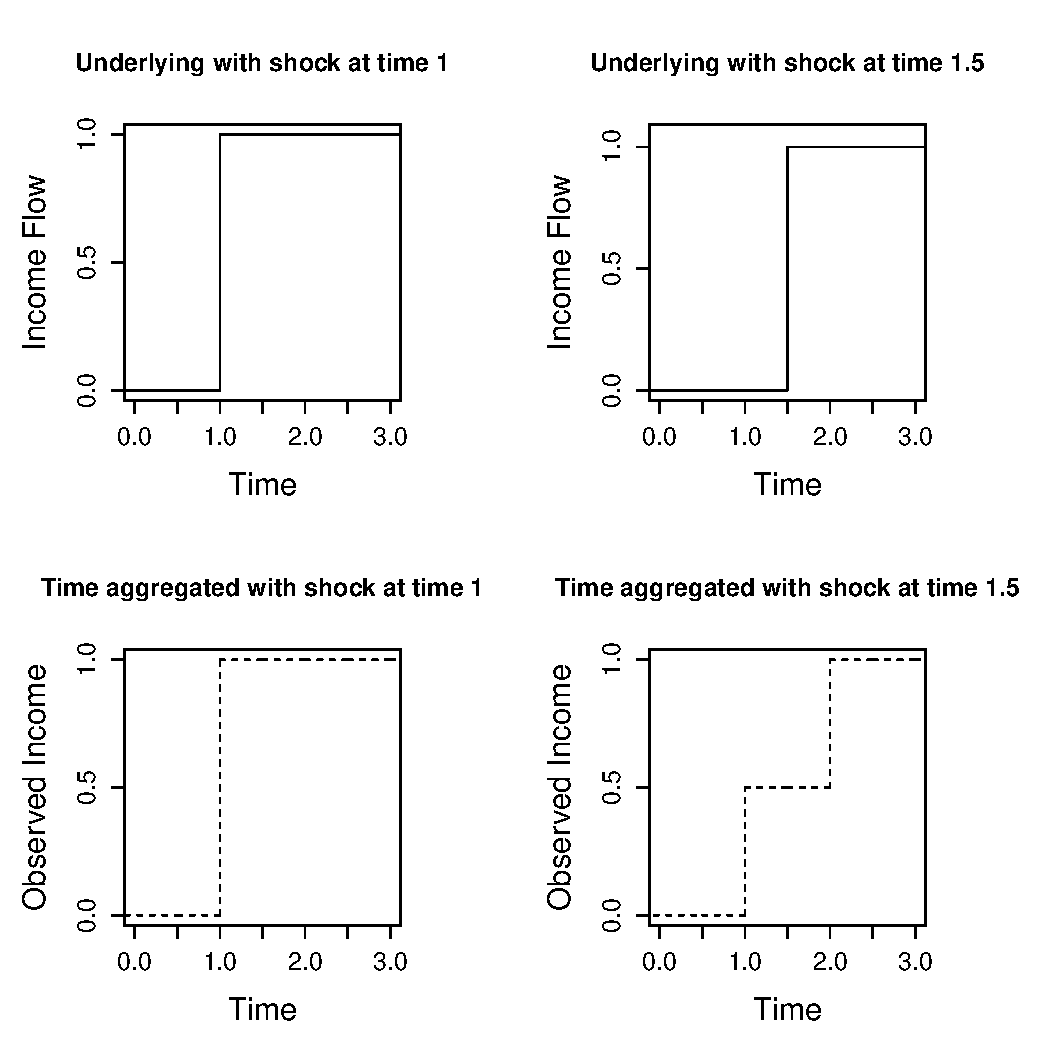
\includegraphics[width=1\textwidth]{TimeAggExample.pdf}
\end{figure}
